\chapter{Funktionsweise von Spark}
\label{chapter:funktionsweise von Spark}


Im vohergehenden Kapitel wurde der Berkeley Data Analytics Stack vorgestellt. Es wurde gezeigt, dass dieser aus einer Reihe von Bibliotheken, Infrastrukturkomponenten und dem eigentlich Kern, Apache Spark, besteht.

In diesem Kapitel werden die grundlegenden Konzepte von Spark vorgestellt und dessen Funktionsweise betrachtet. Einleitend wird gezeigt, wie eine Spark-Infrastruktur aufgebaut sein kann, wie diese intern Abfragen und eigene Spark-Programme verarbeitet und wie der \textit{Spark-Context} sich als Cluster-Repräsentant gegenüber dem Anwender und der API exponiert. Im nächsten Unterkapitel wird die eigentliche Basis von Apache Spark vorgestellt. Spark basiert im Wesentlichen auf einer verteilten Datenstruktur, den \textit{Resilient Distributed Datasets}. Deren Konzept wird sowohl theoretisch, als auch im Anwendungskontext dargestellt. 

Ein weiteres Kernelement der Spark-Implementierung bildet das \textit{In-Memory-Processing} der Daten. Spark ist in der Lage, je nach Konfiguration des Host-Systems, große Teile der Analysen und Verarbeitungen äußerst flexibel im Hauptspeicher durchzuführen und so massive Performanceverbesserungen gegenüber festspeicherbasierter Verarbeitung zu generieren. Hierzu bietet Spark spezielle \textit{In-Memory-Primitives} an. In einem weiteren Unterkapitel werden dieses detailliert vorgestellt. 



\section{Spark im Cluster}
\label{section:spark im cluster}

%Diesen Abschnitt noch mit Referenzen untermauern
Eine große Herausforderung im Umfeld verteilter und nebenläufiger Analyse und Verarbeitung großer Datenmengen stellt der Netzwerkverkehr da. Der klassische Aufbau einer verteilten Anwendung hält die Daten auf einer dafür vorgesehen Plattform im Netzwerk. Häufig ist dies ein dedizierter File- oder Datenbankserver, der mit möglichst großer Bandbreite mit dem Applikationsserver verbunden ist (Vergleich Oracle InfinyBand). 

%Hier muss noch eine Grafik eines herkömmlichen Netzwerks rein
\begin{figure}[htb!]
\centering
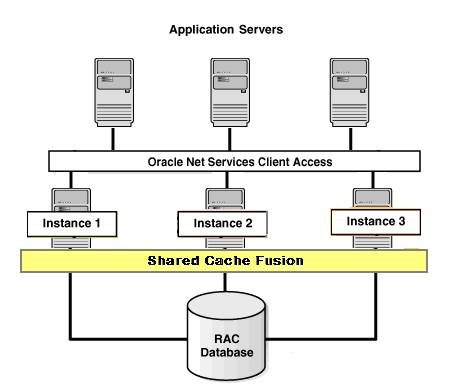
\includegraphics[width=1.0\textwidth]{bilder/oracle_cluster.jpg}
\caption{Aufbau eines Standardcluster im Rechenzentrumsbetrieb mit Application-Server und Oracle Datenbanken \protect\citeint{or14}. }
\label{fig:sparkclustermastermitworker}
\end{figure} 

In diesem Aufbau entsteht in der Regel eine sehr hohe Netzwerklast, da die für die Applikation benötigten Daten dieser zunächst zur Verfügung gestellt werden müssen. 

Spark geht hier einen anderen Weg. Ein Spark-Cluster besteht typischerweise aus einem zentralen \textit{Master} und n \textit{Worker-Nodes}. Diese können aus einfachen Servern bestehen, aber auch aus Clustern von Großrechnern (beispielsweise IBM Z, Oracle Exa). Das Hadoop Distributed File System und Spark skalieren über Cluster beliebiger Größenordnung. Über ein verteiltes Dateisystem werden die Daten auf dem Cluster gehalten und sowohl dem \textit{Master}, als auch den \textit{Worker-Nodes} so zur Verfügung gestellt. 

%Hier Grafik zum Aufbau eines Spark Clusters. 
\begin{figure}[htb!]
\centering
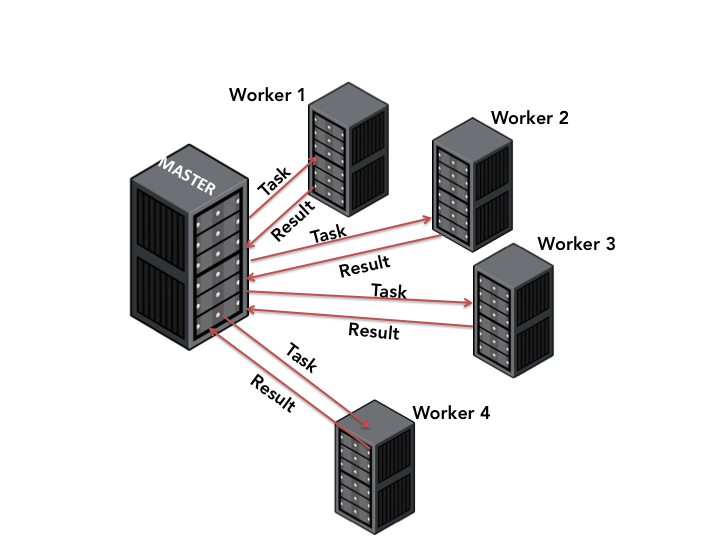
\includegraphics[width=1.0\textwidth]{bilder/spark1.png}
\caption{Clusteraufbau mit Spark mit einem Master und vier Worker-Nodes. }
\label{fig:sparkclustermastermitworker}
\end{figure} 



Spark-Anwendungen laufen als unabhängiges Set von Prozessen auf Cluster-Infrastrukturen. Das Hauptprogramm, der sogenannte \textit{Spark Driver}, instanziert das\textit{ SparkContext-Objekt}, das die einzelnen Prozesse koordiniert. Auf Clustersystemen hält der \textit{SparkContext} die Verbindung zum jeweiligen \textit{Cluster-Ressource-Manager} (Mesos, Yarn), im Standalone-Betrieb instanziert der Context selbst einen Dummy-Manager und allokiert in beiden Fällen die für die Anwendung nötigen Hardware-Ressourcen. Die Cluster-Manager liefern ihren aktuellen Status an Spark zurück und melden Auslastung und Gesundheitszustand der einzelnen Knoten. Über interne \textit{Load-Balancing-Systeme}\footnote{Load-Balancing-Systeme sind Überwachungsmechanismen in verteilten Systemen. Jedes Teilsystem meldet seine eigene Auslastung und seine Verfügbarkeit an den Load-Balancer. Dieser verteilt anstehenden Aufgaben so auf die Ressourcen, dass eine möglichst gleichmäßige Verteilung über die gesamte Infrastruktur möglich ist.} wird ermittelt, welche Worker-Nodes die jeweiligen Tasks aus dem Spark-Kontext zugewiesen bekommen. Der SparkContext repräsentiert sowohl für die Spark-Konsole REPL, als auch in eigenen Spark-Programmen innerhalb der APIs das gesamte Cluster. Dem SparkContext wird bei der Initialisierung über ein Konfigurationsobjekt mitgeteilt, welche Ressourcen ihm für das aktuelle Programm zur Verfügung stehen. Die Entscheidung, welche, der initial zur Verfügung gestellten Nodes oder Ressourcen des Clusters von Spark wann in Anspruch genommen werden, obliegt der Kombination aus Spark und \textit{Cluster-Ressource-Manager}. 

%gesamten Abschnitt mit Referenzen belegen!    

%fußnote nochmal überdenken

\begin{figure}[htb!]
\centering
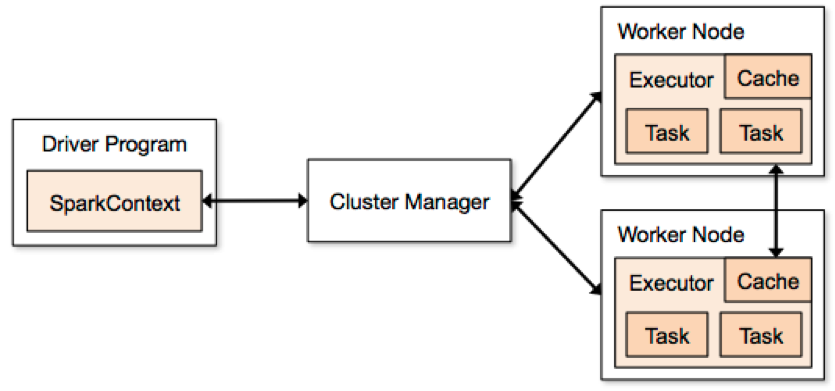
\includegraphics[width=1.0\textwidth]{bilder/3_2_cluster.png}
\caption{Clusteraufbau mit Spark \protect\citeint{sp14}}
\label{fig:sparkcluster}
\end{figure} 





Wenn ein SparkContext initialisiert wurde, installiert der Spark sogenannte \textit{Executors} auf sämtlichen Worker-Nodes des Clusters. Der Applikationscode wird nun als JAR\footnote{Ein JAR (Java ARchive) ist ein gepacktes und auf einer Java Virtual Machine ausführbares (Java, Scala, Clojure) Programmpaket, häufig inklusive der benötigten Bibliotheken.} direkt an die Executors verteilt und dieser anschließend durch entsprechende Tasks ausgeführt. 



  
\section{Das Konzept der Resilient Distributed Datasets}
\label{section:rdd}

Die Resiliient Distributed Datasets (RDD) sind das eigentliche Kernelement von Apache Spark. Hierbei handelt es sich um fehlertolerante, parallele Datenstrukturen, die dem Anwender erlauben, Zwischenergebnisse explizit im Hauptspeicher zu halten, ihre Partitionierung zu steuern, um Daten bewußt an bestimmten Stellen halten zu können und diese mittels umfangreichen Operatoren zu manipulieren  \citelit{rdd12}. Das Konzept der RDDs entspricht prinzipiell den Views\footnote{Eine View ist in einem relationalen Datenbanksystem die Ergebnismenge einer persistierten Datenbankabfrage auf bestimmte Daten. Diese lässt Abfragen analog zu einer gewöhnlichen Tabelle zu.} in relationalen Datenbanksystemen. Werden die RDDs für weitere Zugriffe persistiert, enspricht dies dem Prinzip der Materialized Views\footnote{Materialized Views entsprechen bei Abfragen den regulären Views. Allerdings wird hier im Gegensatz zu den Views bei Zugriff keine Abfrage auf die zugrundeliegenden Tabellen durchgeführt. Stattdessen sind die Daten als Kopie in eigenen Datenbankobjekten persistent vorhanden.}.  

RDDs werden mittels deterministischer, paralleler Operationen erstellt, den sogenannten \textit{Transformationen}. Im Fehlerfall, also wenn beispielsweise ein \textit{Node} im Cluster ausfällt, können die RDDs automatisch an Hand der durchgeführten Regeln neu aufgebaut werden. Deshalb merken sich die RDDs die Transformationen, die zu ihrem Aufbau geführt haben und können so verlorene Datenstrukturen schnell rekonstruieren. Die \textit{Resilient Distributed Datasets} können ausschließlich durch Transformationen, wie beispielsweise \textit{map, filter, join}, etc., aus Daten aus dem Dateisystem oder aus anderen, bereits vorhandenen RDDs erzeugt werden, oder durch Verteilen einer Object-Collection in der Driver-Applikation. Diese Datenstrukturen müssen nicht persistiert werden, da sie für einen Partitionierung ausreichende Informationen über ihre Erstellungsregeln und die entsprechenden Datensätze enthalten, das sogenannte \textit{Lineage} \citelit{rdd12}.   

Da es sich bei RDDs prinzipiell um Scala-Collections handelt, können diese auch direkt in Scala-Code eingebunden und verarbeitet werden, oder interaktiv über die Scala-Konsole REPL genutzt werden. Aber auch für Java und Python bietet Spark APIs an. Für weitere Sprachen wie R oder Clojure existieren Wrapper-Frameworks, welche die RDDs und ihre Operationen verfügbar machen.  RDDs können nur durch grobgranulare, deterministische Transformationen, erstellt werden.

WIe eingangs beschrieben, verfügen die Anwender von Spark über die Kontrolle der Aspekte \textit{Persistence} und \textit{Partitioning} \citelit{rdd12}. Mit der Persistence lässt sich festlegen, welche RDDs wiederverwendet werden sollen, also welche RDDs nach welcher Strategie persistiert werden sollen. Das Partitioning legt fest, nach welchen Kriterien die RDDs geteilt und über das Cluster verteilt werden sollen, also beispielsweise sortiert nach bestimmten Keys. Die Optimierung der Partitionierung ist unter Anderem wichtig für Join-Operationen. Je nach Partitionierungsstrategie kann dies erhebliche Unterschiede in Laufzeit und Ressourcennutzung bedeuten.  

RDDs können prinzipiell auf drei Arten gespeichert werden \citeint{sp14}:
\begin{itemize}
		\item Als deserialisiertes Java-Objekt im Speicher der JVM – dieses Variante bietet die beste Performance, da die Objekte sich direkt im JVM-Heap befinden
		\item Als serialisiertes Java-Objekt direkt im Speicher – dieses Verfahren ist speicher-effizienter, aber schlechter in der Zugriffsgeschwindigkeit
		\item Im Dateisystem – diese Variante ist erwartungsgemäß die langsamste, jedoch nötig, wenn die RDDs zu groß für die Haltung im RAM sind. 		
\end{itemize}	


\begin{tabular}{ l l c | r |}
\hline
test1 test2 test3
\end{tabular}


Wie in Abbildung \ref{section:rdd} dargestellt, werden die Daten bei einer Verarbeitung durch Spark zunächst aus dem HDFS geladen, in Resilient Distributed Datasets (RDD) verpackt, und dann im Hauptspeicher für Verarbeitung- oder Analysefunktionen zur Verfügung gestellt. Abfragen werden direkt entweder via Scala REPL oder SQL-artige Abfragen zur Laufzeit, über Batch-Jobs oder via Spark Streaming/Storm an die im RAM befindlichen RDDs geleitet.

\begin{figure}[htb!]
\centering
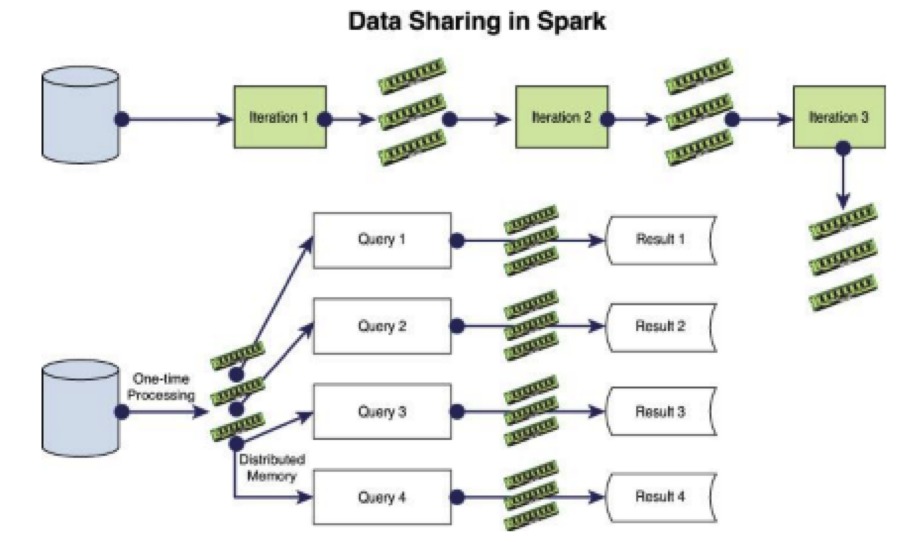
\includegraphics[width=1.0\textwidth]{bilder/3_spark.png}
\caption{Schematische Darstellung der Funktionsweise von Spark \protect\citeint{va14}}
\label{fig:sparkfunkt}
\end{figure}



\section{Die In-Memory-Primitives von Spark}
\label{section:rdd}


\section{Die Spark-Console REPL}
\label{section:rdd}


\section{Die Spark APIs}
\label{section:rdd}


























